
%Copyright (C) 2016 by Krishneel@JSK Lab, The University of Tokyo

\documentclass{standalone}
\begin{document}

\section{task3}
\subsection{Platforms}
For task 3, we applied two kinds of UAVs to challenge the task. The general UAV called "hawk" as shown in Fig.\ref{fig:task3-hawk}, which is similar to the one used in task 1, and the transformable aerial robot with multilink which is called "Hydrus"(Fig.\ref{fig:task3-hydrus}). As described in Fig.\ref{fig:task3-hydrus-platform},tThe hardware platform of "Hydrus" envolves the controller for joints which enables the stable aerial transformation.

\begin{figure}[h]
  \begin{center}
    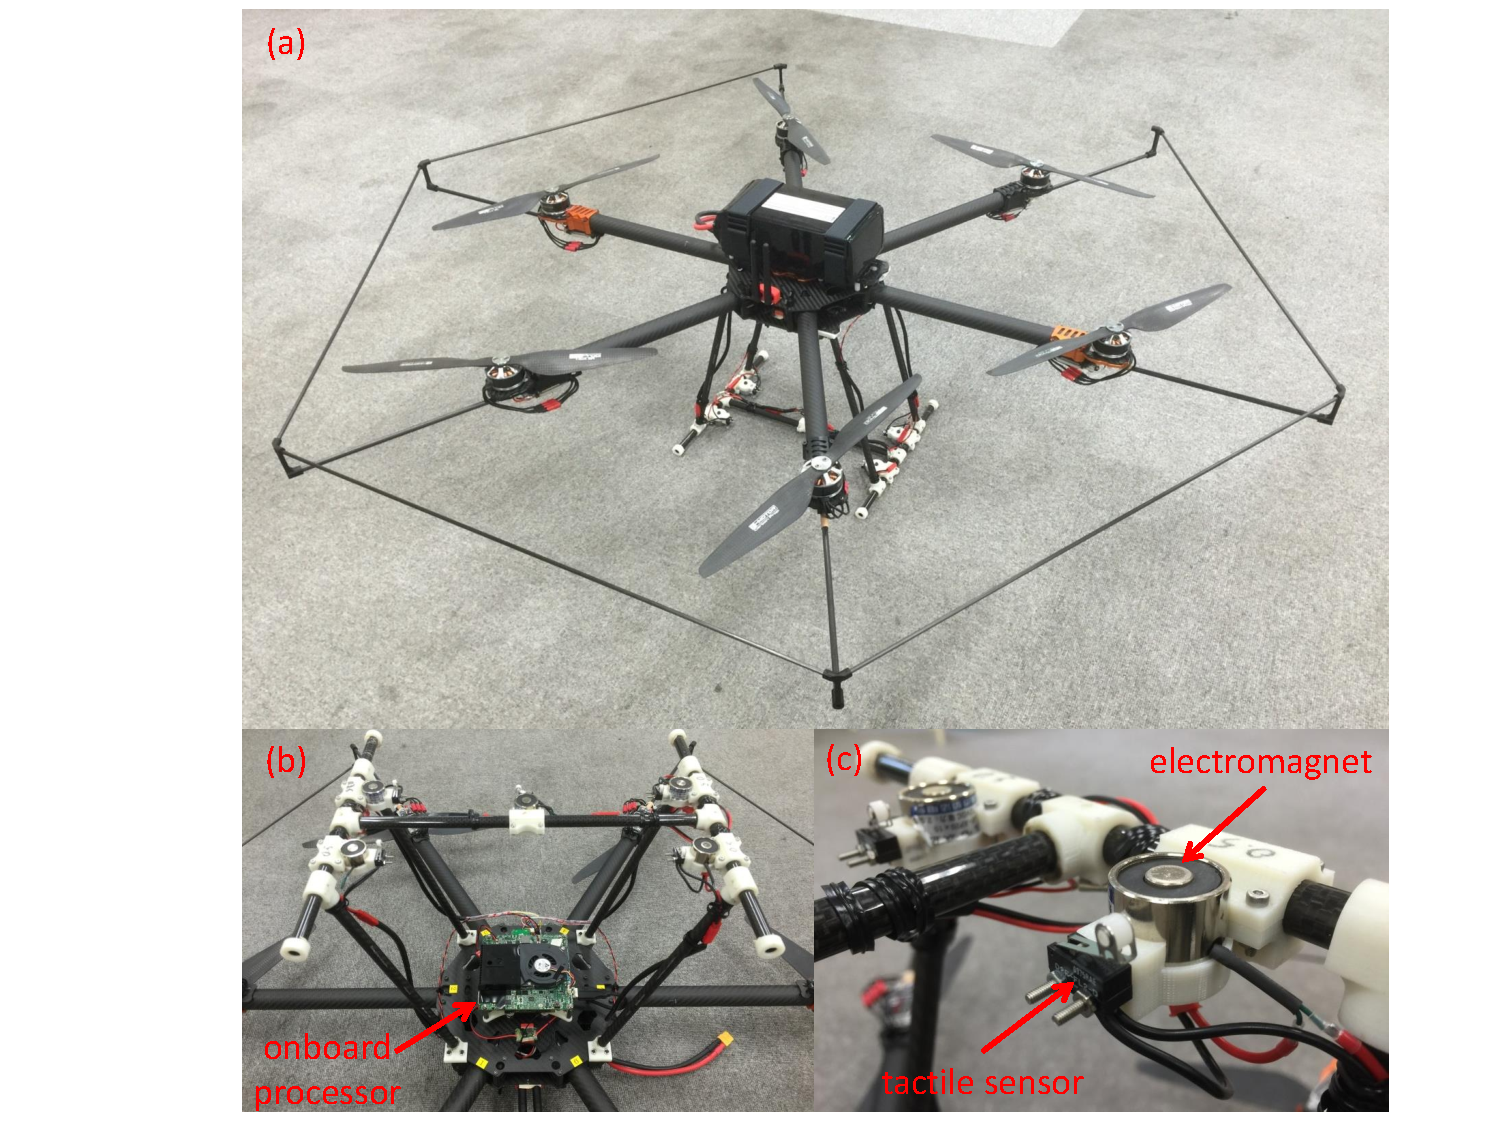
\includegraphics[clip,  bb=115 4 666 535,  width=\columnwidth]{sections/task3/images/task3-tarrot810.pdf}
    \caption{Image of task3 Hawk}
    \label{fig:task3-hawk}
  \end{center}
\end{figure} 

\begin{figure}[h]
  \begin{center}
    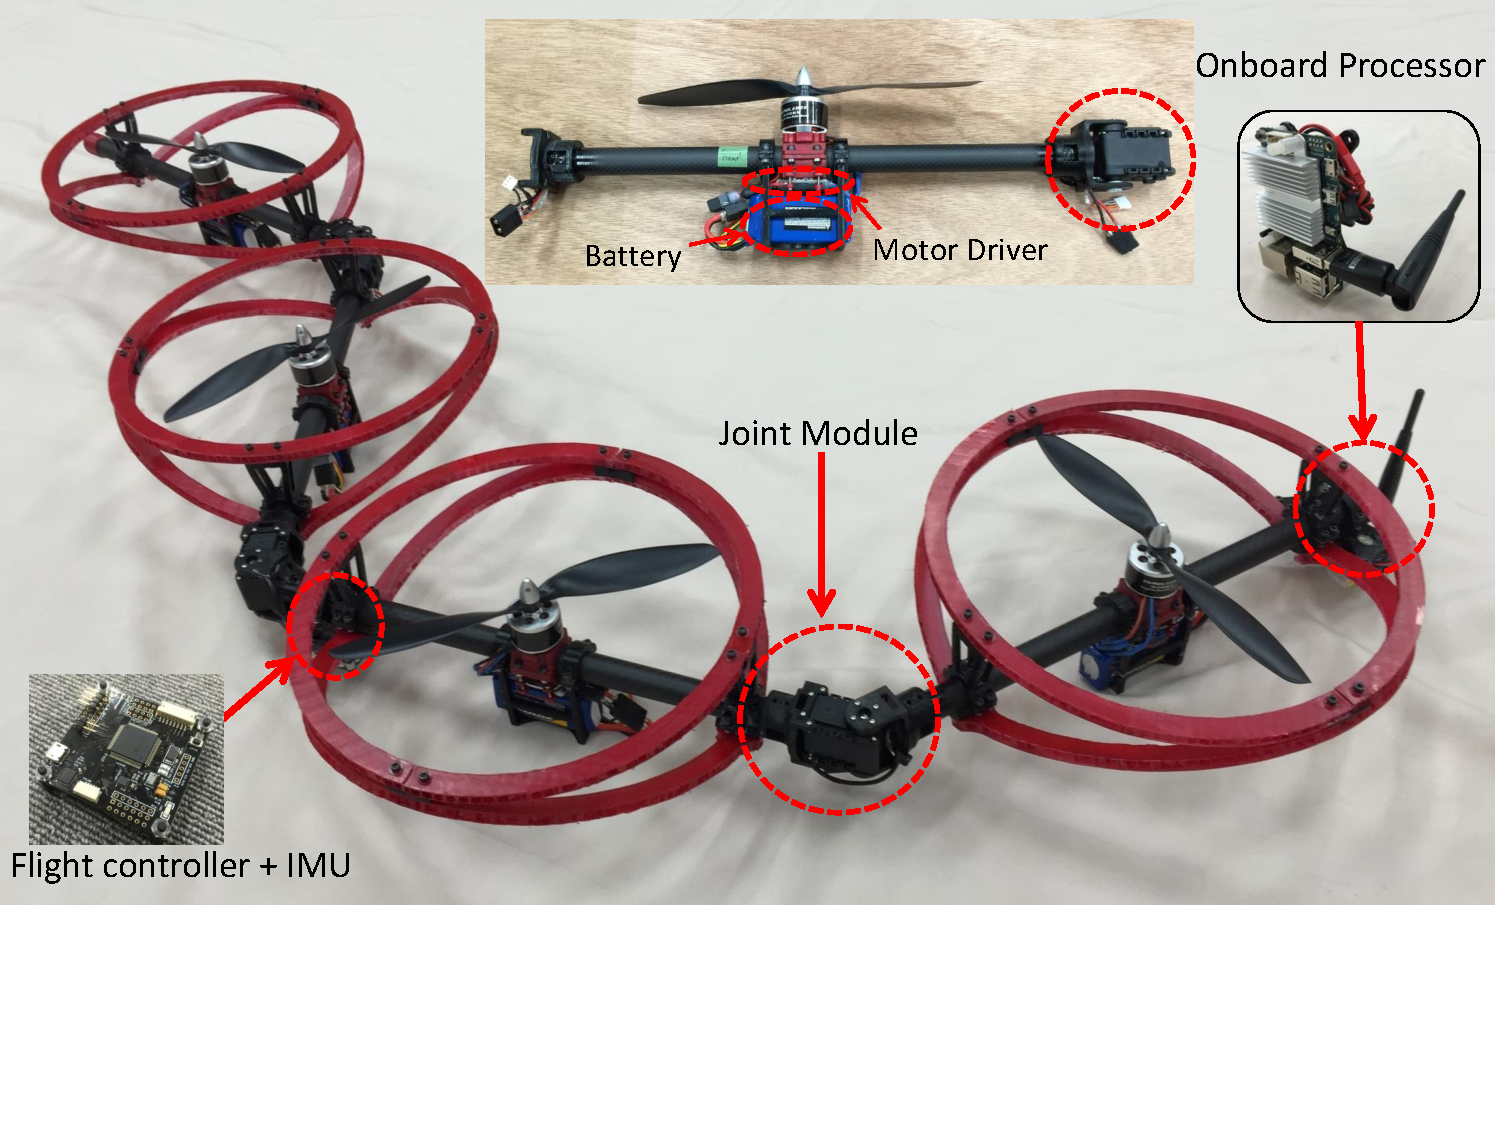
\includegraphics[clip,  bb=0 105 720 535,  width=\columnwidth]{sections/task3/images/task3-hydrus.pdf}
    \caption{Image of Hydrus}
    \label{fig:task3-hydrus}
  \end{center}
\end{figure} 

\begin{figure}[h]
  \begin{center}
    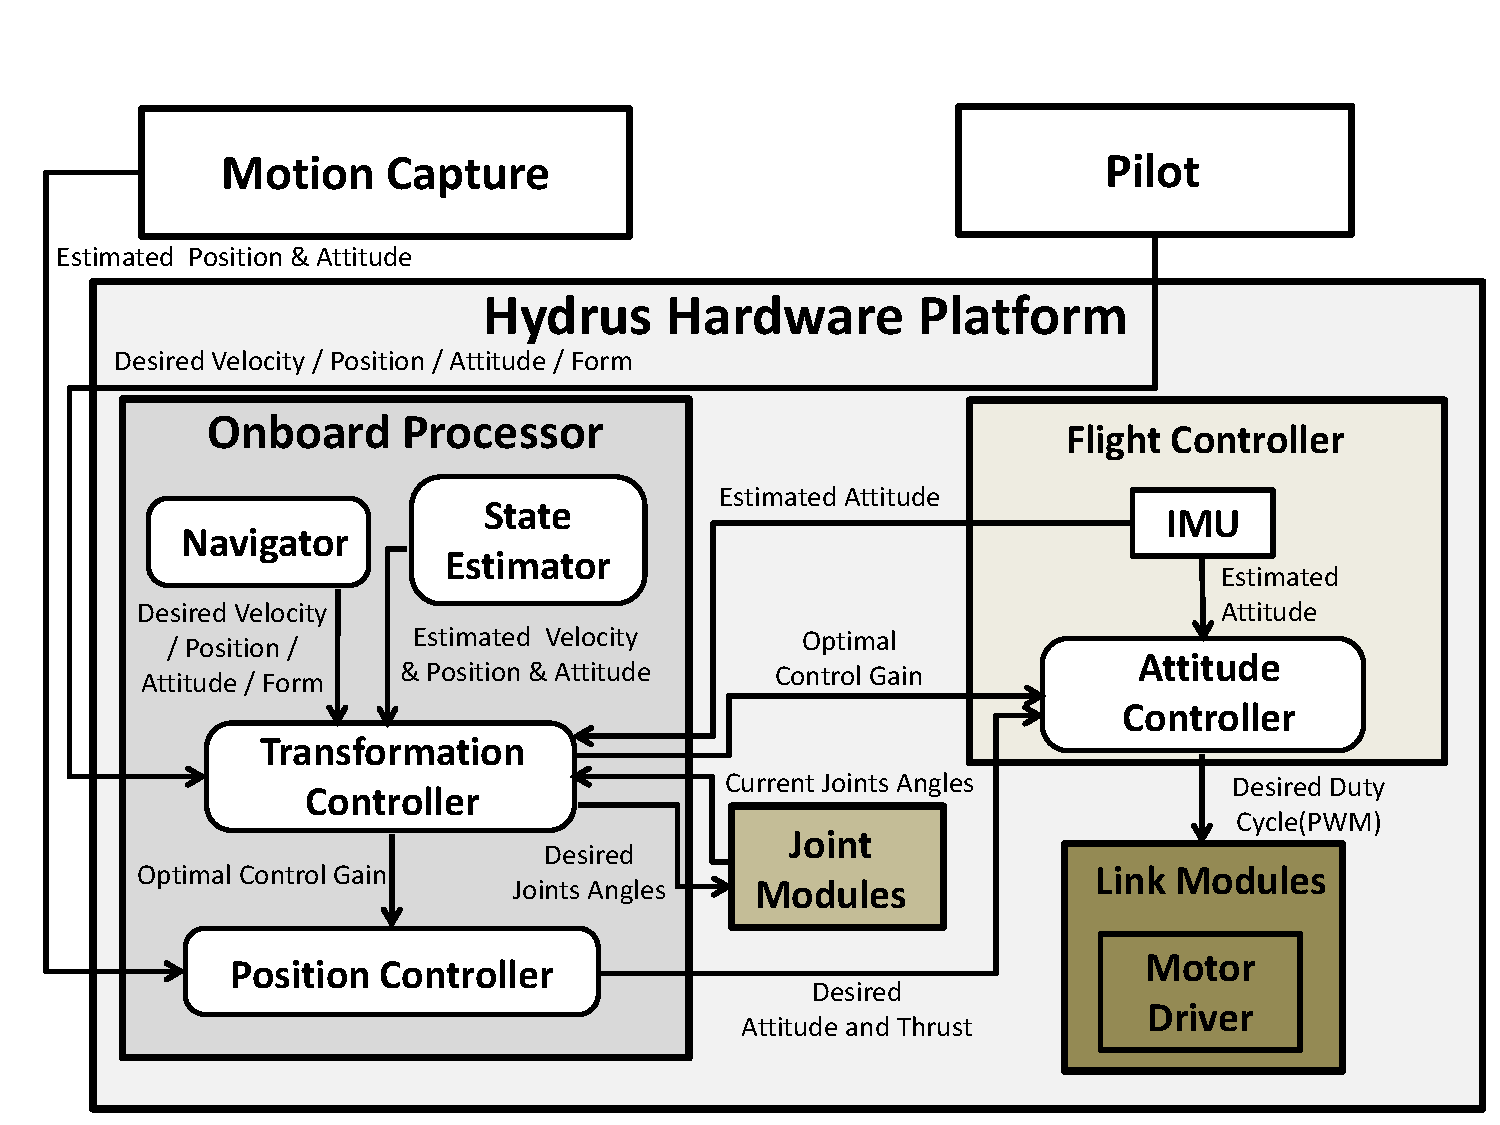
\includegraphics[clip,  bb=0 0 720 540,  width=\columnwidth]{sections/task3/images/hydrus-platform.pdf}
    \caption{Hardware platform of task3 Hawk}
    \label{fig:task3-hydrus-platform}
  \end{center}
\end{figure} 



Although the flight control algorithms between "Hawk" and "Hydrus" are fundamentally different, we use the smae flight controller board which is build by ourselves. We additionally designed another PCB board for controlling the eletromagnet module which can generate the suction force up to 20[N]. We equipped 5 eletromagnet in the UAV and build the attachment with tactile sensors as shwon in Fig.\ref{fig:task3-hawk}(c). The electro-magnet moudle control board is connected to the flight  controller board unit through CAN bus.

For the transformable UAV, we introduce the prototype which contains four links and three servo joints. The modularization of the whole platform is achieved by distributing the power and control system to each link with excpect of flight controller and sensors. Therefore, it becomes easier to the change the amount of rotors, according to the application of the flight.

\subsection{Aerial Manipulation Strategy}
For each type of UAV, we develop different piccking method. For "hawk" type UAV, we appy the magnetic force to absorb the ferrous object as shown in Fig.\ref{fig:task3-hawk-manipulation}. When the contact between the bottom of landing gear and object occurs, the tactile sensor provides certain signal, leading the actication of the eletromagnet module. We have achieve to the pick and carry the object inder indoor enviroment using motion capture system, which confirm the validty of the eletro-magnet based manipulation strategy. The cylinder type object is created according to the regulation description.

\begin{figure}[h]
  \begin{center}
    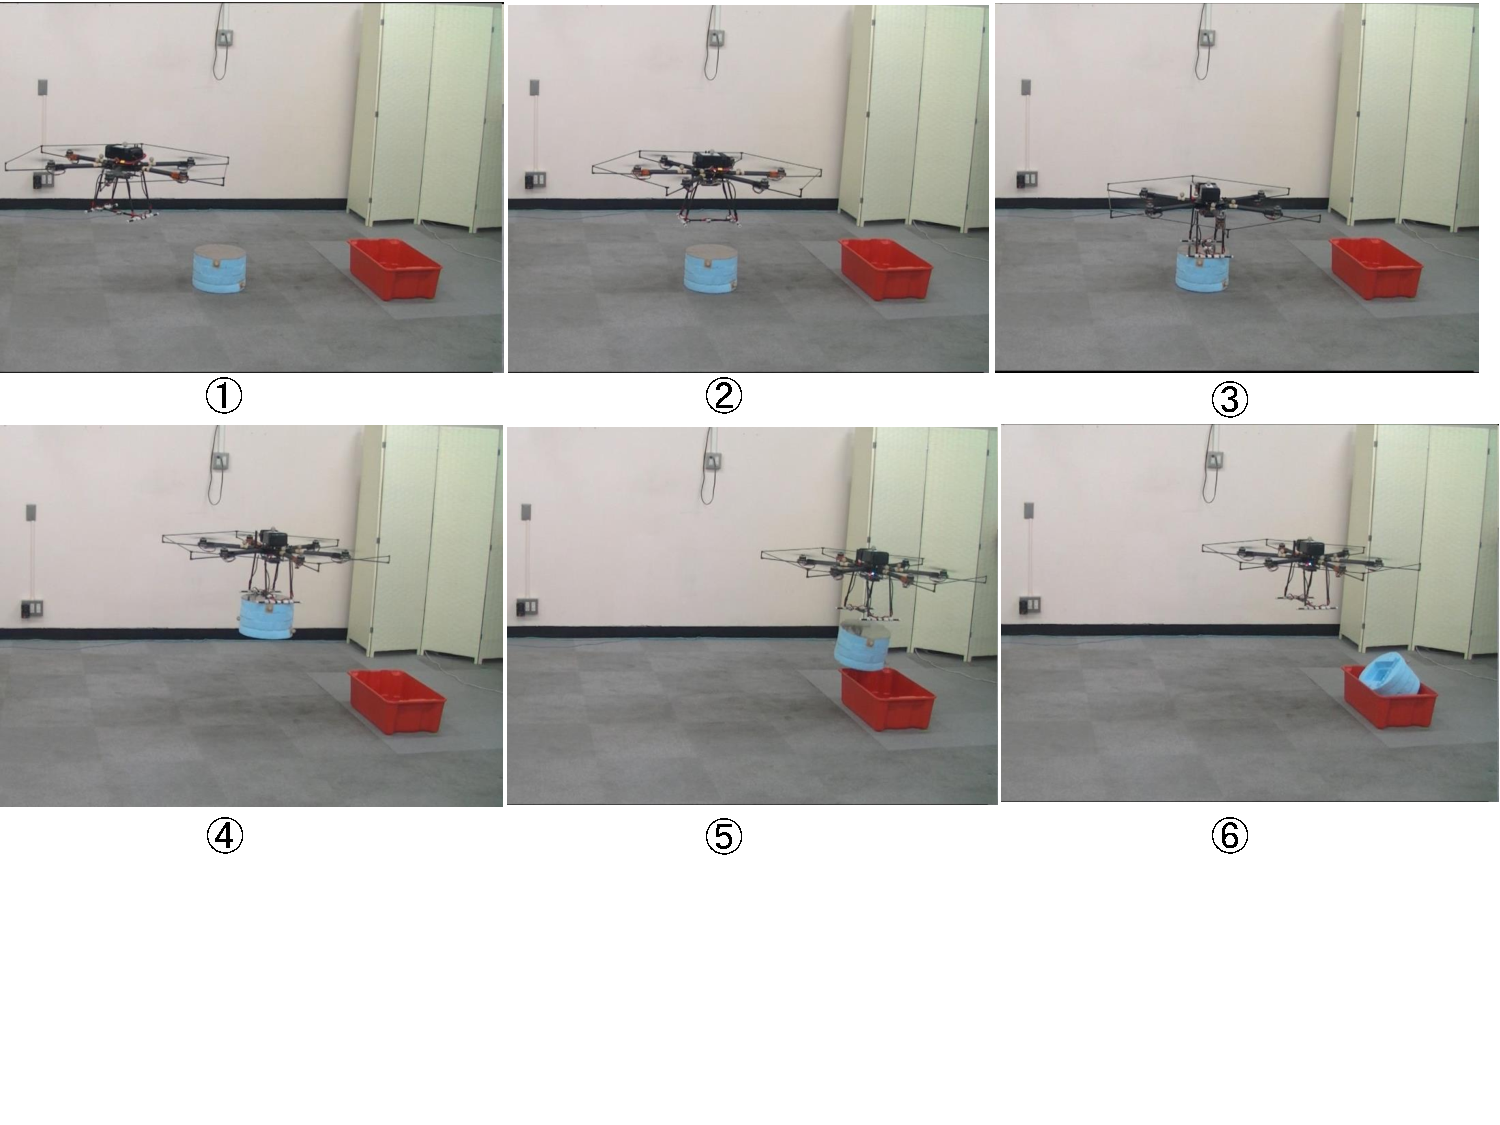
\includegraphics[clip,  bb=0 110 720 540,  width=\columnwidth]{sections/task3/images/task3-tarrot810-manipulation.pdf}
    \caption{Aerial manipulation method of Hawk}
    \label{fig:task3-hawk-manipulation}
  \end{center}
\end{figure} 

On the other hand, the object transporation based on the whole-body-manipulation strategy using "Hydrus" is also acheived as shown in Fig.\ref{fig:task3-hydrus-manipulation}. The grasping control is developped  based on the torque feedback from each joint. 

\begin{figure}[h]
  \begin{center}
    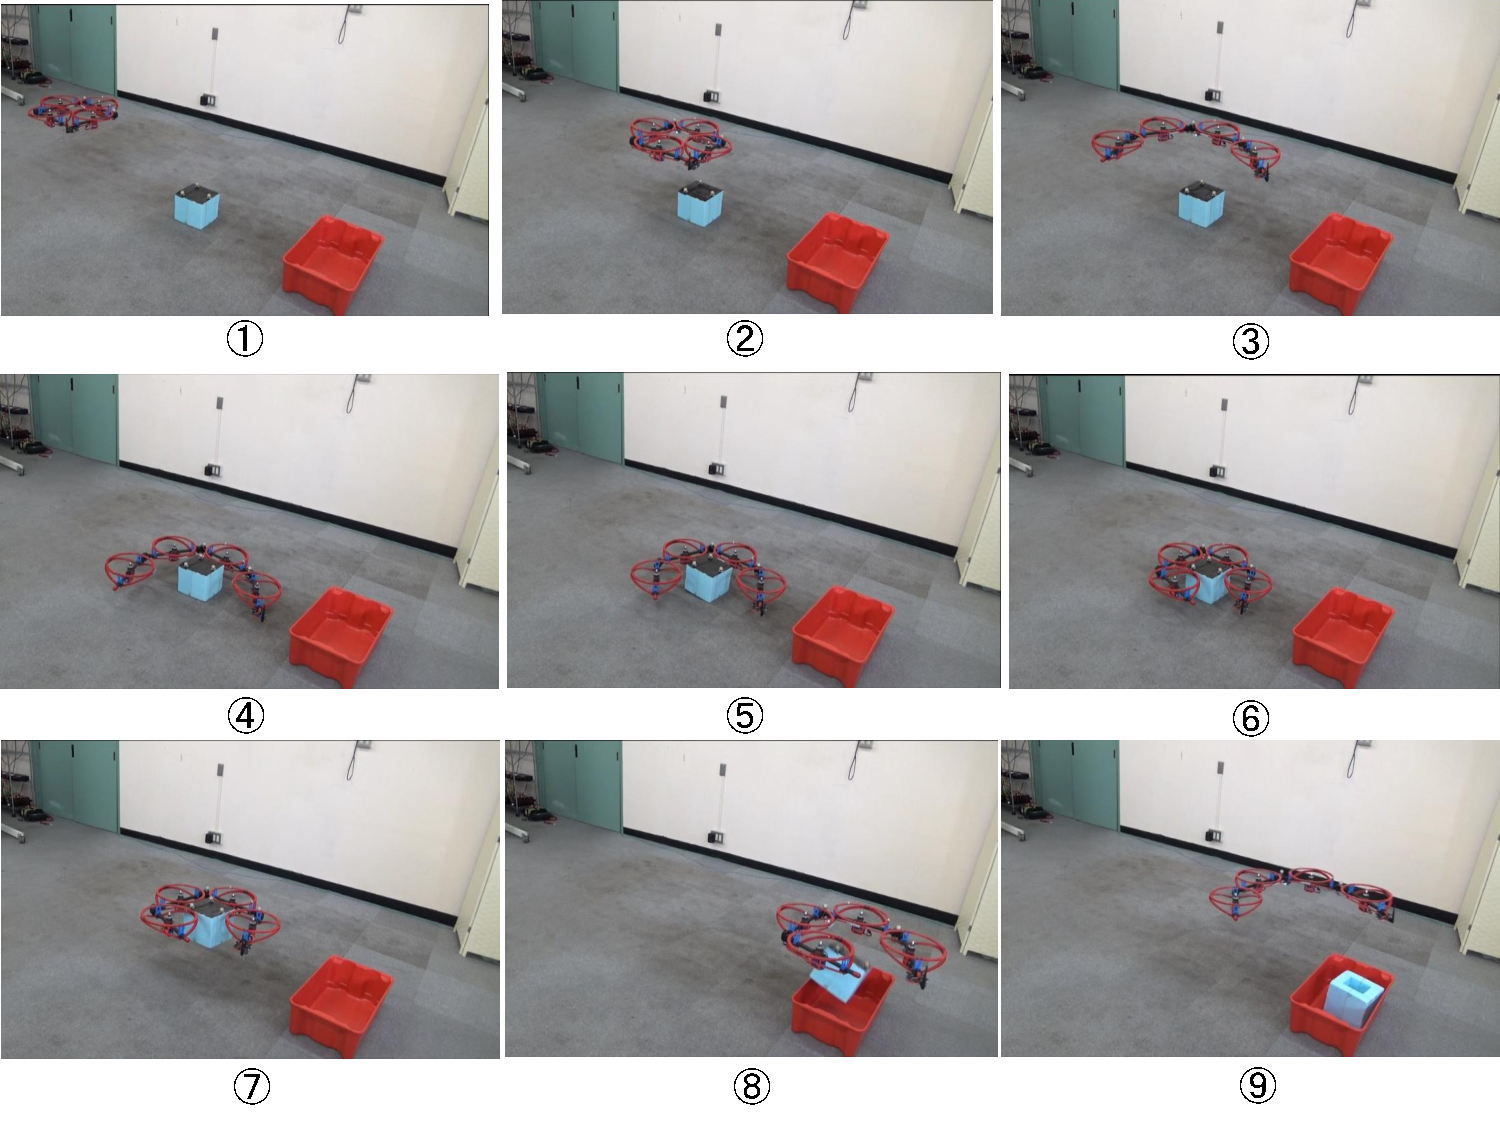
\includegraphics[clip,  bb=0 0 720 540,  width=\columnwidth]{sections/task3/images/task3-hydrus-manipulation.pdf}
    \caption{Aerial manipulation method of Hydrus}
    \label{fig:task3-hydrus-manipulation}
  \end{center}
\end{figure} 

\subsection{Software}
Just like other tasks the softwares are build on ROS environment and some functionalities are shared from task 1. Point Cloud and OpenCV libraries are used for visual perception. % target detection and motion planning are different.

\subsubsection{General Approach}
%The software system is based on ROS(Robot Operation System). We write our algorithm to the every single node and communicate with each node. 
Basically for task 3, we divide the task into three states: Search, Pick and Place. The UAVs are always within these three states and the states automatically transferred to the next one if the certain condition is satisfied as illustrated in Fig. \ref{t3}A. In "Search" state, the drone will traverse to the center of the arena and randomly generate a search end-point, the treasure detector will work when the drone is searching, once the object is detected and locked, a pick motion will be generated in the "Pick" state, the UAV will open the Elec-Magnet and moving approach to the treasure. The transfer state signal depends on the trigger of the tactile sensor, once the Elec-Magnet catch the treasure, the UAV enters "Place" state, it will directly fly to the placing zone and find the box to place the treasure. After release the treasure upon the place box, the UAV re-enter the "Search" state and loops until task is completed.

 \begin{figure}%[hb]
    \begin{center}
      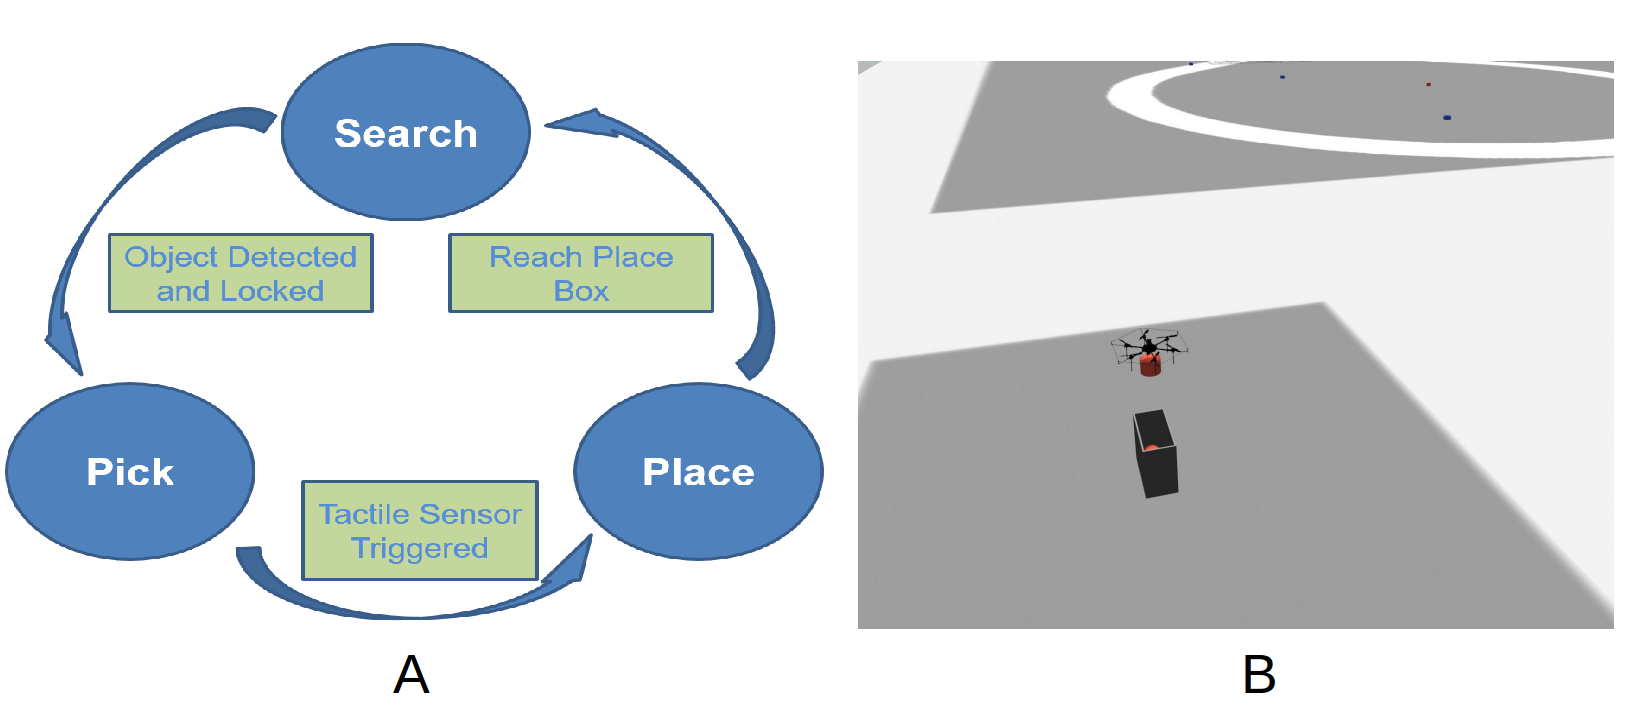
\includegraphics[keepaspectratio=true, width=1\linewidth, height=0.30\textheight]{img//task3.png}
    \end{center}
    \caption{Task 3 Demonstration}
    \label{t3}
  \end{figure}


\subsubsection{Treasure Detection}
As the treasures have distinct color features compared to the ground, we firstly used a simple detection method to localize the treasure. 
The inputs are 3D points $p_i$ from the Stereo sensor and the RGB image projection to the ground by the projection matrix computed using the known camera parameters. %We first apply 
HSI color filter is applied to obtain to 3D point candidates of treasure from the point cloud data. Next we apply Euclidean clustering to the filtered point cloud $P_{hsi}$. Euclidean clustering technique can organize points into clusters with respect to the distance feature in 3D space. For $\forall p_i, p_j \in P_{hsi}$, clusters $O_i = \{p_i \in P_i\}$ and $O_j = \{p_j \in P_j\}$ are obtained by:
\begin{equation}\label{eq3-1}
min||p_i - p_j|| \geq d_{threhold} 
\end{equation}

When we get all the clusters, we apply a simple tracker to every cluster center and as we continue to detect the same cluster over time space, the weight of the tracker is increased to boost the confidence of tracking. For clusters that are not always detected the confidence are slowly decreased and removed from the treasure candidates vector. The UAV will lock the cluster candidate when the weight is large enough and switch into the "Pick" mode to approach the treasure.

\subsubsection{Simulation}
We first perform full automatic simulation in gazebo environment as shown in Fig.\ref{t3}B. To fully simulate the real scene, we add noise and outliers to the detection. In simulation, the UAV takes almost 70$seconds$ to detect, pick and place a single object. In future we will use three UAVs in coordination to complete the task which will not only decrease the time but also can be used to transport larger treasures which a single UAV might not be able to lift.
% we believe we can do that better. 
For real robot, we tested with tele-operation control, both Hawk and transformable UAV can grasp the treasure, pick and place into a specificed box. We are planing to perform more test on the real robot to justify the detection and motion planning algorithm in the simulation as part of the future work.


\subsection{Future Plan}
The future work on hardware platform for task 3 contains the improvement of the structural strength, as well as the enhancement of the modularization of link system by using CAN communication network. We will also continue to validate the performance of the eletromagnet module, and the  collaboration between the eletromagnetic force and whole-body-manipulation will be developped for the "Hydrus."

The future work on software for task 3 involves the outdoor expeirment with acutal robot to test the performance of both eletromagnet module and whole-body-manipulation. Further more, we will focus on the collaborative motion for picking up the large object using two or three UAV simultaneously, as well as the swarm control strategy while searching object.


\end{document}
